\documentclass[final]{beamer}

\usepackage[
  size=custom,
  width=84.1,
  height=118.9,
  scale=1.0
]{beamerposter}

\makeatletter
\def\input@path{{isba2026_poster/}}
\makeatother
\usepackage{beamerthemeucscisba}

\graphicspath{
  {isba2026_poster/figures/generated/}
  {isba2026_poster/figures/frozen/}
  {figures/generated/}
  {figures/frozen/}
  {Figures/multivariate_synthesis_by_cutoff/}
  {../Figures/multivariate_synthesis_by_cutoff/}
}

\hypersetup{
  colorlinks=true,
  urlcolor=ExalTeal,
  linkcolor=ExalTeal
}

\title{Dynamic Bayesian Quantile Synthesis for Medium-Range River-Flow Forecasting}
\author{Antonio Aguirre \and Raquel Prado \and Bruno Sanso}
\institute{Department of Statistics, University of California, Santa Cruz}

\begin{document}
\begin{frame}[t]

\begin{tikzpicture}[remember picture,overlay]
  \fill[SoftPanel] (current page.north west) rectangle ([yshift=-11.8cm]current page.north east);
  \fill[ExalTeal] (current page.north west) rectangle ([yshift=-0.35cm]current page.north east);
\end{tikzpicture}

\vspace*{0.15cm}
\begin{minipage}{\textwidth}
  {\postertitlefont\bfseries\color{PosterNavy}\RaggedRight
  Dynamic Bayesian Quantile Synthesis for Medium-Range\\[-0.05em]
  River-Flow Forecasting\par}
  \vspace{0.45cm}
  {\posterauthorfont\color{PosterInk}
  Antonio Aguirre \quad Raquel Prado \quad Bruno Sanso\par}
  \vspace{0.15cm}
  {\postersmallfont\color{MutedGrey}
  Department of Statistics, University of California, Santa Cruz \quad
  Contact: \href{mailto:jaguir@ucsc.edu}{jaguir@ucsc.edu}\par}
  \vspace{0.55cm}
  {\postersubtitlefont\bfseries\color{ExalTeal}\RaggedRight
  Across five rolling origins, exAL-M-T1 has the lowest 28-day CRPS at four cutoffs;
  AL-M-T1 leads at the 2022-12-25 cutoff.\par}
\end{minipage}

\vspace{1.0cm}

{\posterbodyfont
\begin{columns}[T,totalwidth=\textwidth]

\begin{column}{0.275\textwidth}

\begin{posterpanel}{Forecasting Problem}
River-flow decisions need predictive distributions, not only point forecasts.
The challenge is that useful information arrives from non-exchangeable sources:
USGS observations, retrospective hydrologic products, GloFAS and NWS forecast
ensembles, and hydrometeorological covariates.

\minirule
\begin{posterbullets}
  \item Forecast quality varies with source, lead time, and hydrological regime.
  \item Retrospective products help learn historical source discrepancies.
  \item Forecast products enter only through information available at the origin.
  \item Evaluation is on held-out USGS observations on the $\log(1+Q)$ scale.
\end{posterbullets}
\end{posterpanel}

\begin{posterpanel}{Information Sources}
\begin{posterbullets}
  \item \textbf{Observed target:} USGS daily San Lorenzo River flow.
  \item \textbf{Historical alignment:} retrospective products from external agencies.
  \item \textbf{Forecast inputs:} ECMWF/GloFAS and NOAA/NWS forecast products.
  \item \textbf{Transfer covariates:} precipitation, soil moisture, and GDPC.
  \item \textbf{Forecast output:} a synthesized posterior predictive distribution.
\end{posterbullets}

\vspace{0.25cm}
\begin{softcallout}
{\bfseries Key design choice.} The external products are combined through
source-specific discrepancy states rather than treated as one homogeneous ensemble.
\end{softcallout}
\end{posterpanel}

\begin{posterpanel}{Validation Design}
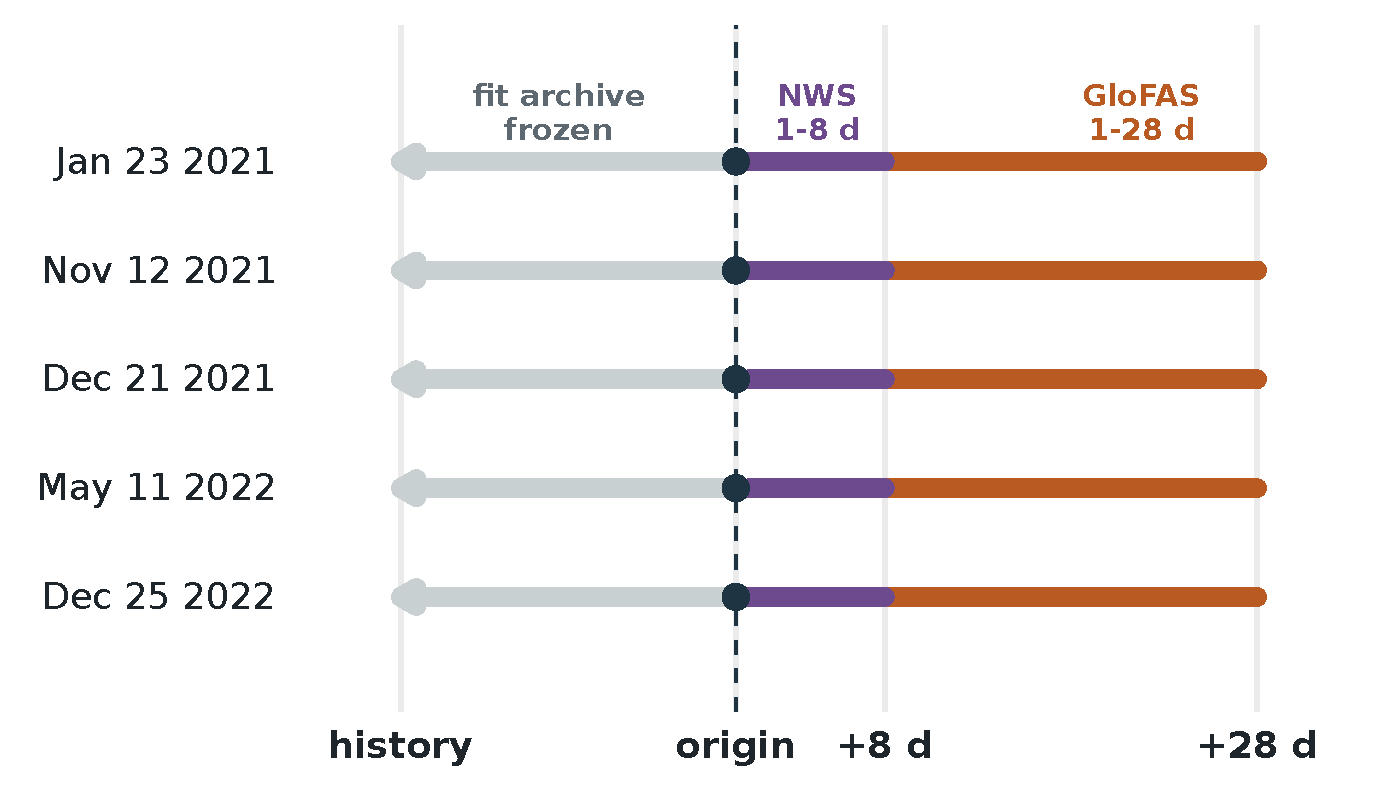
\includegraphics[width=\linewidth]{rolling_origin_timeline.pdf}
\smallcaption{At each origin, the model is fit only through the cutoff. The
28-day forecast window is verified against post-cutoff USGS observations; the
first eight days define the horizon-compatible NWS comparison.}
\end{posterpanel}

\begin{posterpanel}{Model Label Decoder}
\begin{tabular}{@{}p{0.20\linewidth}p{0.72\linewidth}@{}}
\toprule
\textbf{Part} & \textbf{Meaning} \\
\midrule
$L$ & likelihood: N, AL, or exAL \\
$S$ & synthesis scope: univariate U or multivariate M \\
$T$ & transfer in forecast window: T0 drops, T1 retains \\
\bottomrule
\end{tabular}

\vspace{0.25cm}
\tagpill{ExalTeal}{exAL-M-T1}
\quad
extended likelihood, multivariate synthesis, retained forecast-window transfer.
\end{posterpanel}

\end{column}

\hfill
\begin{column}{0.395\textwidth}

\begin{posterpanel}{Dynamic Quantile Synthesis}
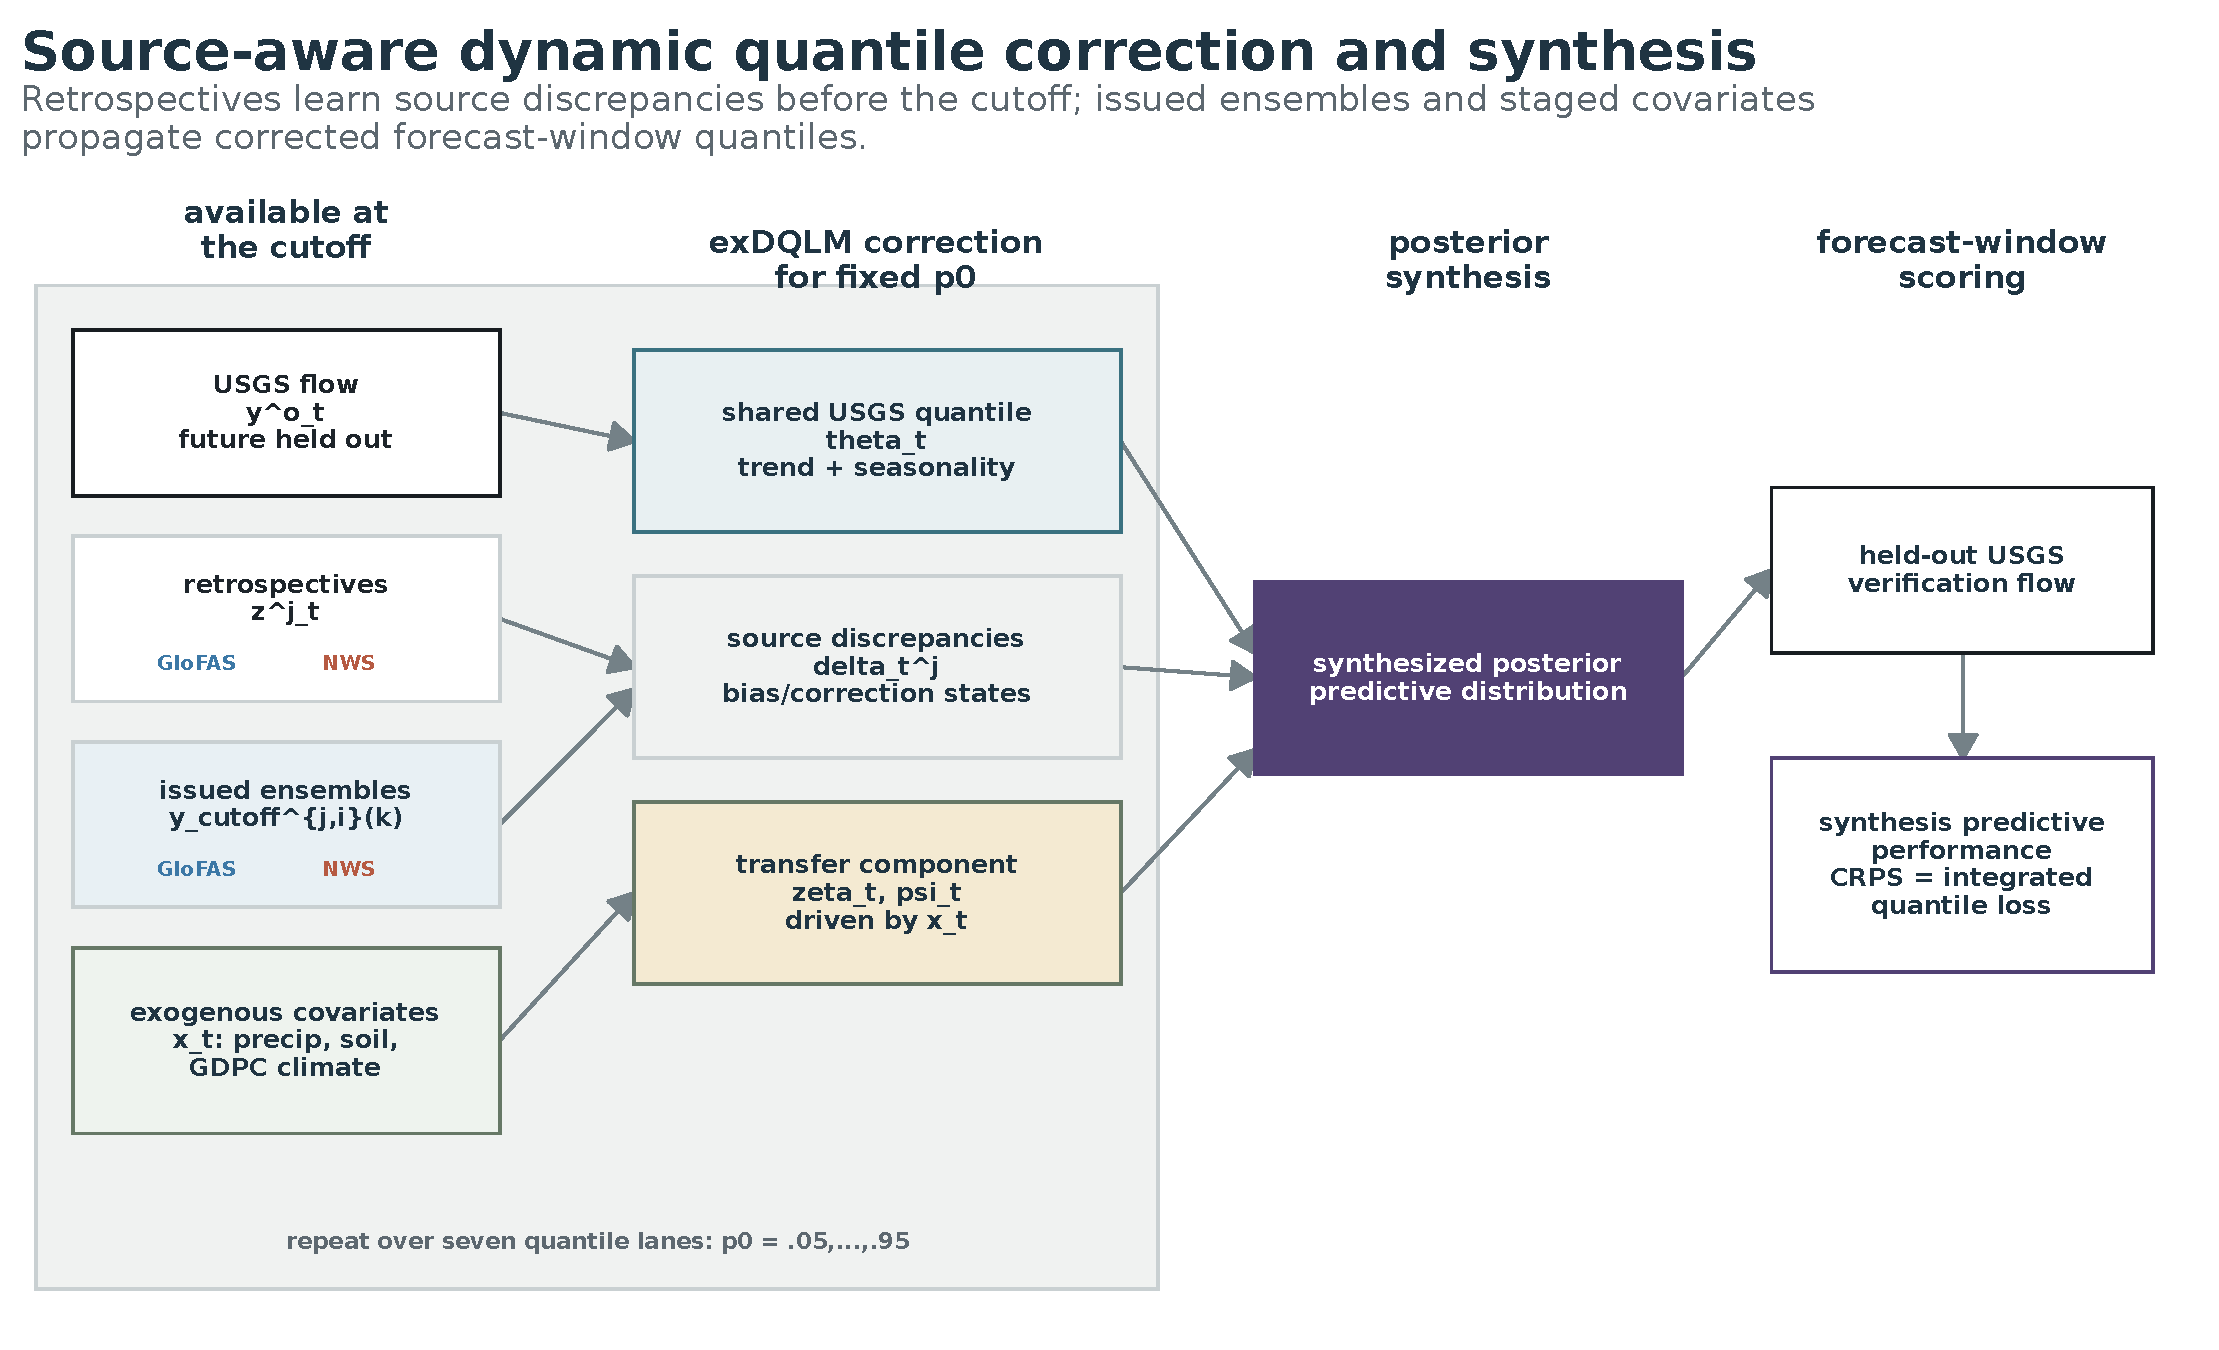
\includegraphics[width=\linewidth]{model_schematic.pdf}
\smallcaption{For each target quantile, a shared latent river-flow quantile
process is combined with source discrepancy states, trend and seasonal dynamics,
and a retained forecast-window transfer component. Quantile-specific posterior
forecasts are then synthesized into one predictive distribution.}
\end{posterpanel}

\begin{posterpanel}[colback=white,colframe=ExalTeal,boxrule=1.05pt]{Main Five-Cutoff Result}
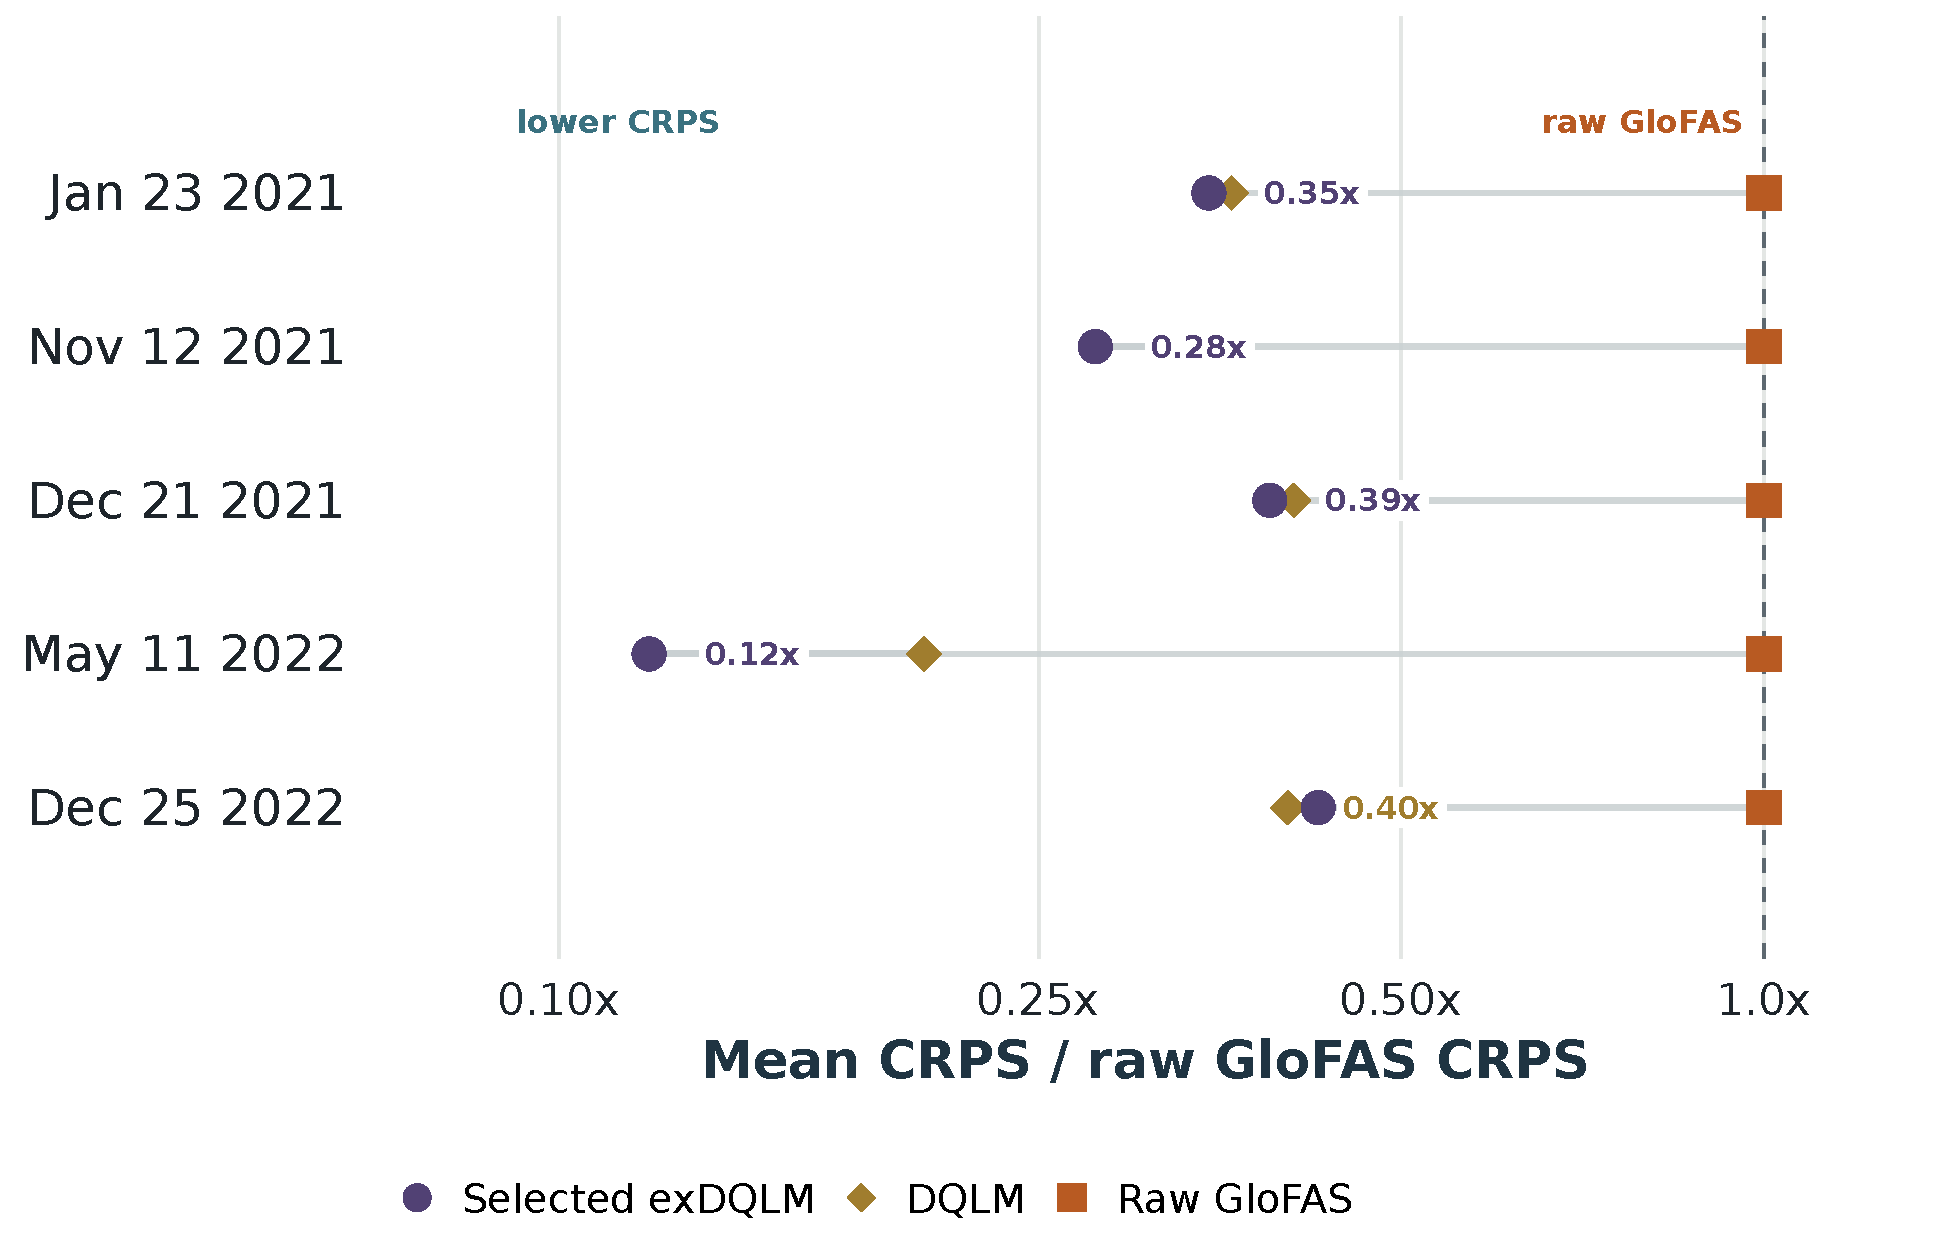
\includegraphics[width=\linewidth]{crps_28d_poster.pdf}

\vspace{0.25cm}
\begin{softcallout}
\evidencecaption{Main message.}
The selected extended-likelihood multivariate active-transfer model
\textbf{exAL-M-T1} has the lowest 28-day CRPS at the first four rolling origins.
The final origin is the important exception: \textbf{AL-M-T1} is lower at
2022-12-25.
\end{softcallout}
\end{posterpanel}

\begin{posterpanel}{Why the Pattern Matters}
\begin{posterbullets}
  \item The strongest corrected forecasts are the multivariate active-transfer
  variants, which combine the observation channel with external sources.
  \item The result is cutoff-specific rather than a universal model ranking.
  \item Raw GloFAS is shown as the 28-day raw product reference; raw NWS belongs
  in the separate eight-day horizon comparison.
\end{posterbullets}
\end{posterpanel}

\end{column}

\hfill
\begin{column}{0.275\textwidth}

\begin{posterpanel}{NWS Horizon Nuance}
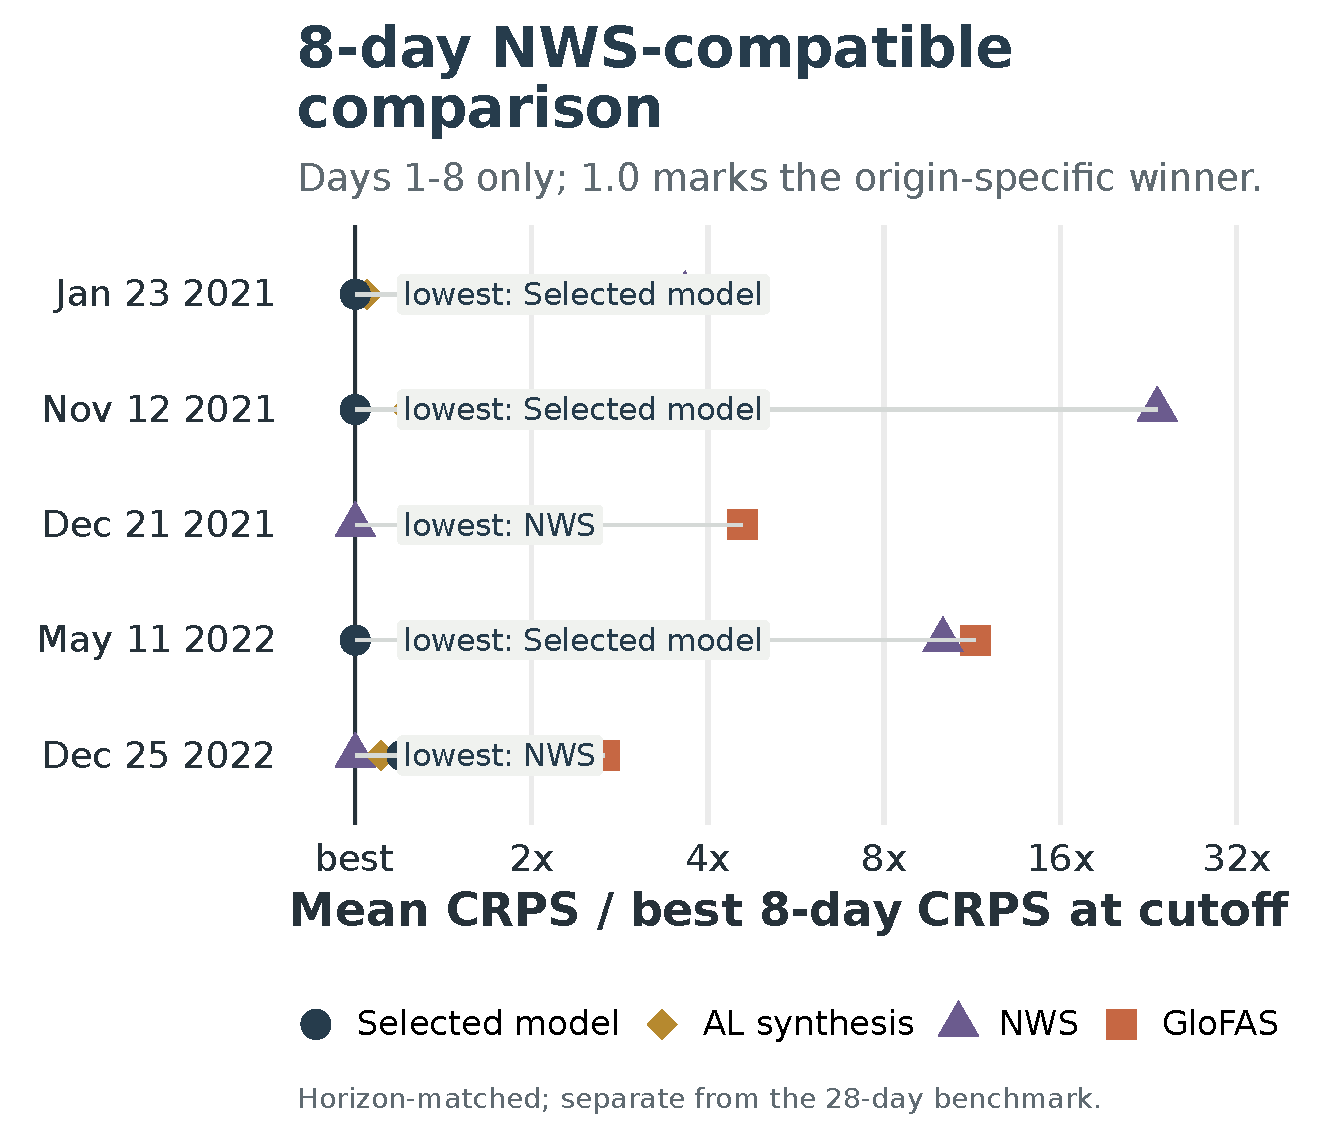
\includegraphics[width=\linewidth]{crps_8d_nws_poster.pdf}
\smallcaption{NWS has eight valid daily leads for these origins. This panel is
therefore the direct NWS comparison; it should not be read as the 28-day
medium-range benchmark.}
\end{posterpanel}

\begin{posterpanel}{Illustrative Forecast Window}
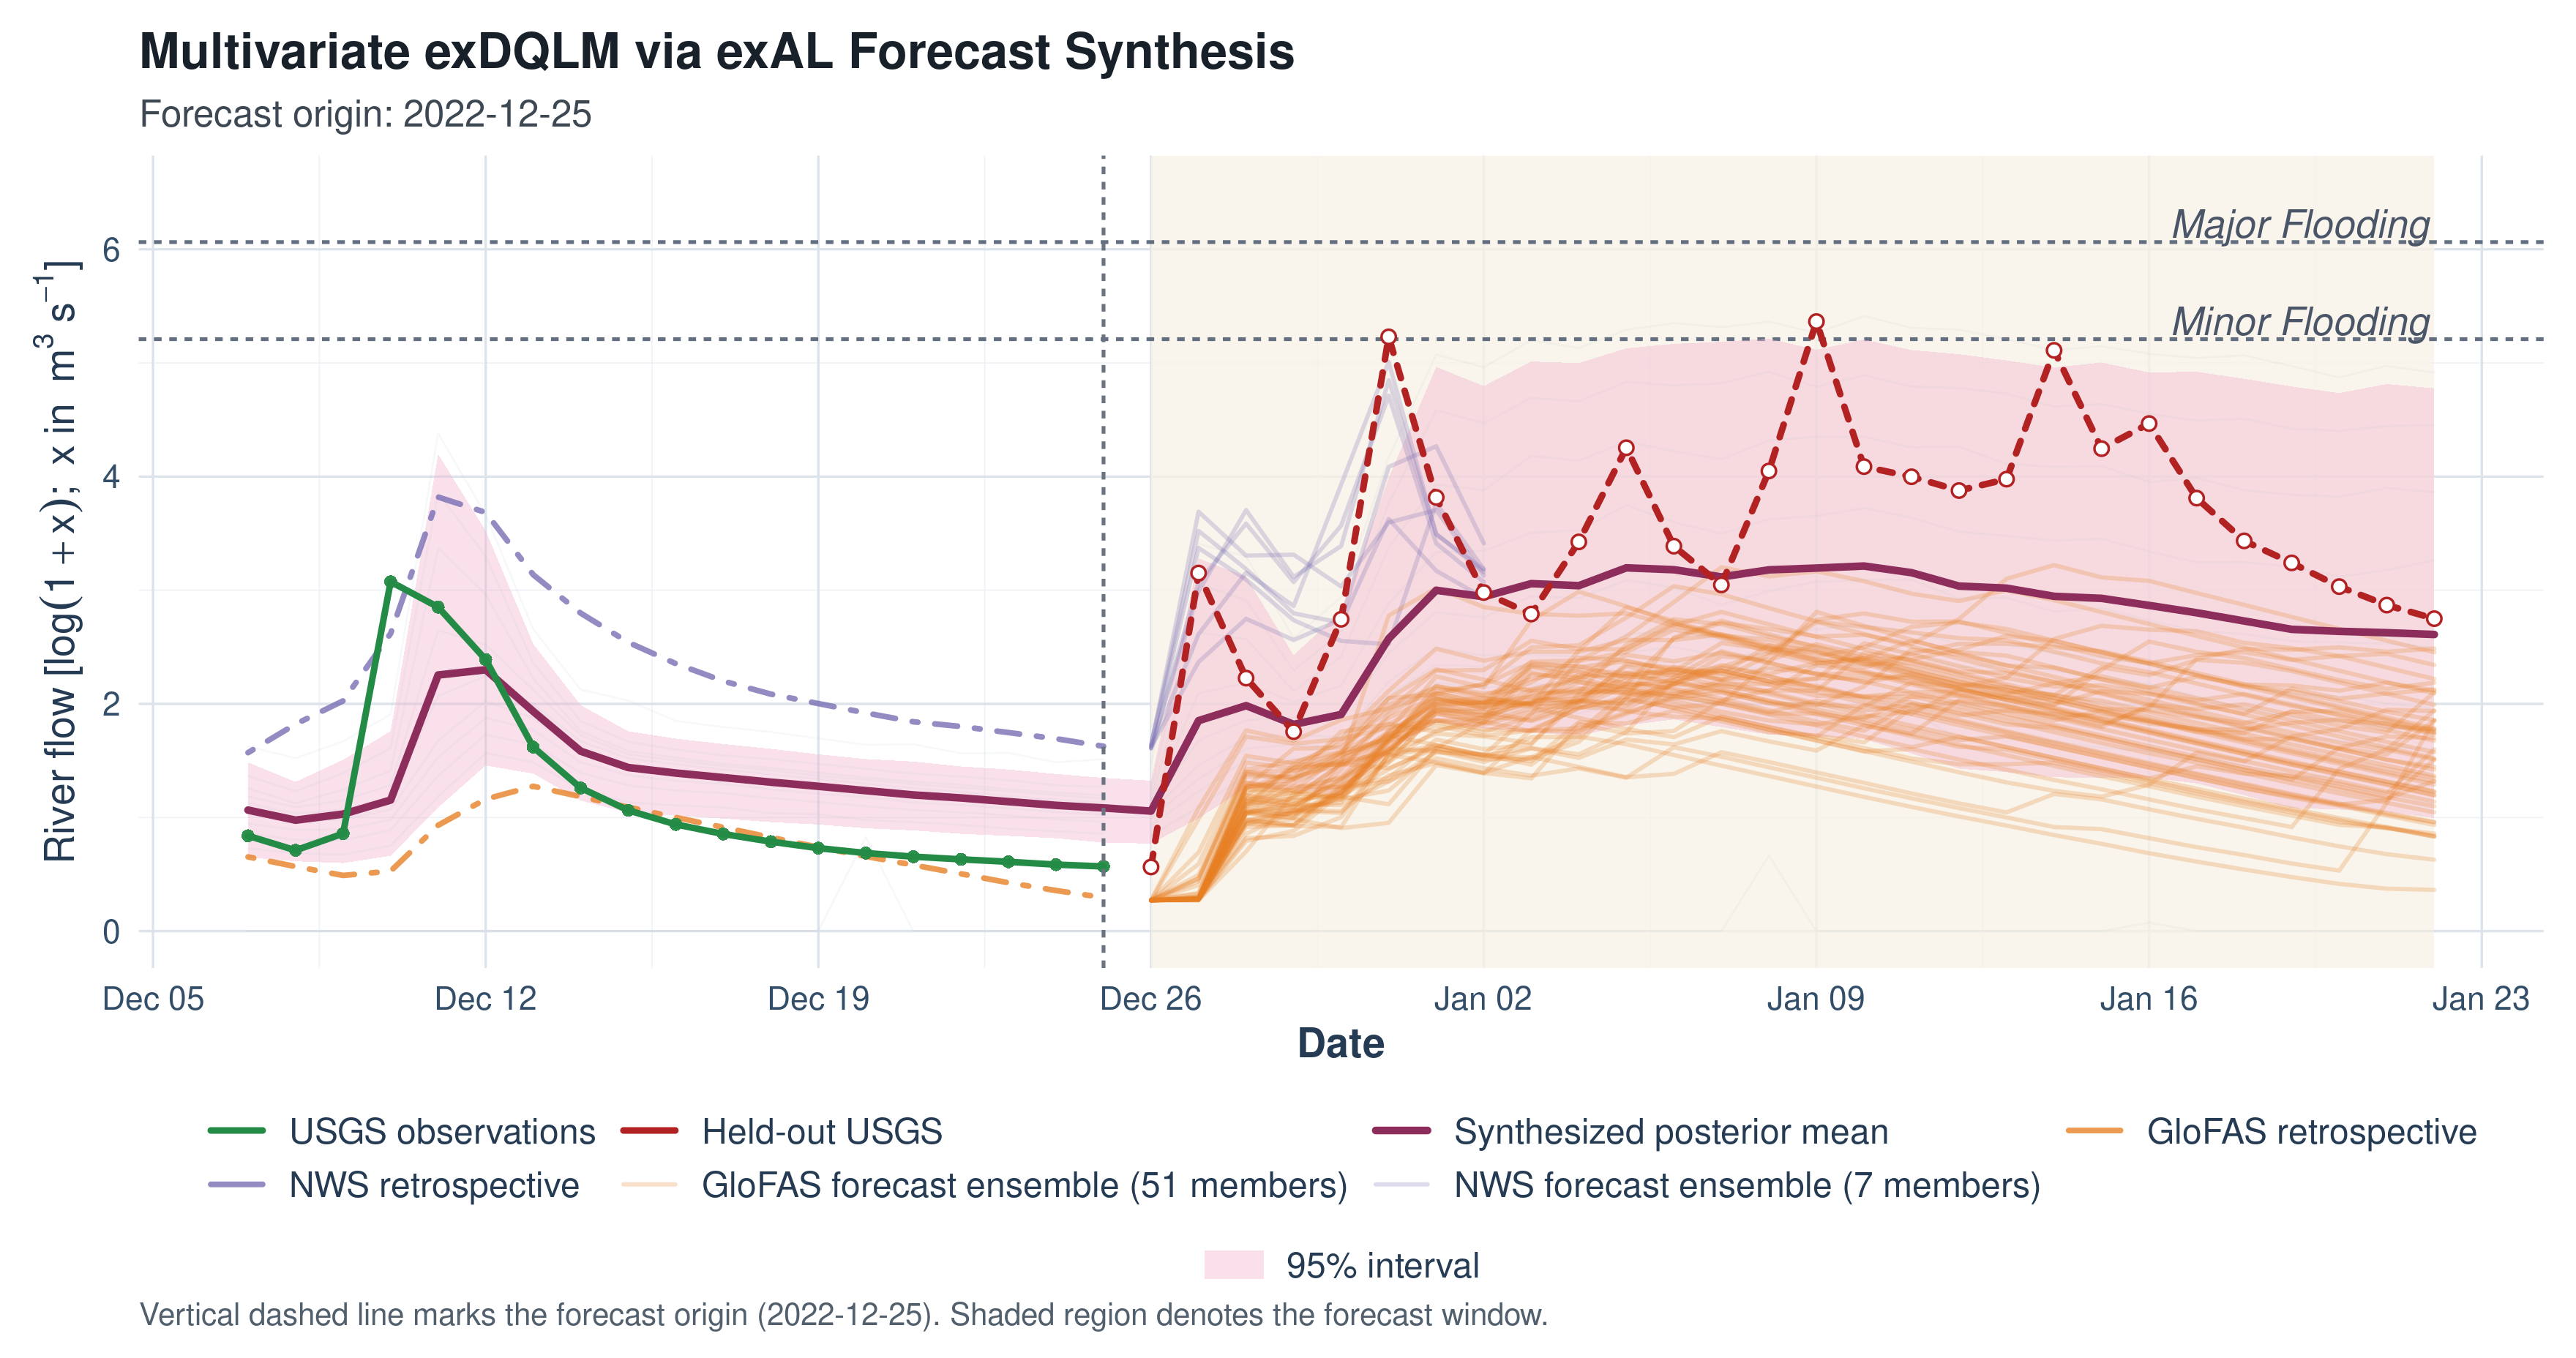
\includegraphics[width=\linewidth]{cutoff_2022_12_25_multivariate_synthesis_with_reference_ensembles.png}
\smallcaption{Representative 2022-12-25 exAL-M-T1 synthesis with reference
forecast products. This display illustrates the selected model at one origin;
aggregate validation is the five-cutoff CRPS comparison.}
\end{posterpanel}

\begin{posterpanel}{Takeaway and Limits}
\begin{posterbullets}
  \item Dynamic Bayesian quantile synthesis gives a coherent way to correct and
  combine heterogeneous hydrologic forecast sources.
  \item The current frozen manuscript evidence supports exAL-M-T1 as the
  selected extended-likelihood multivariate reference, with the final-cutoff
  AL-M-T1 nuance kept explicit.
  \item The evaluation uses five flood-relevant rolling origins, not a dense
  continuous hindcast.
  \item The ongoing discount/epsilon screen is excluded until any replacement is
  formally promoted through the article and corrections workflow.
\end{posterbullets}

\vspace{0.25cm}
\begin{goldcallout}
\textbf{Next methodological steps:} joint treatment of multiple quantiles, richer
discrepancy dynamics, and spatial extensions across nearby basins.
\end{goldcallout}
\end{posterpanel}

\begin{posterpanel}{Reproducibility}
\begin{posterbullets}
  \item Frozen article artifacts: generated TeX tables, figure manifests, and
  five-cutoff CRPS validation sources.
  \item Workflow code: \href{https://github.com/AntonioAPDL/Project1}{github.com/AntonioAPDL/Project1}.
  \item Poster figures are generated from frozen manuscript tables, not
  hand-entered into the poster source.
\end{posterbullets}
\end{posterpanel}

\end{column}
\end{columns}
}

\vspace{0.7cm}
{\posterbodyfont
\begin{posterpanel}[colback=SoftPanel,colframe=PanelLine]{Three Takeaways}
\begin{columns}[T,totalwidth=\linewidth]
\begin{column}{0.31\linewidth}
\tagpill{ExalTeal}{1}
\quad \textbf{Source-aware correction.}\par
\vspace{0.15cm}
The model treats observations, retrospective products, forecast products, and
covariates as distinct information channels rather than a single exchangeable
ensemble.
\end{column}
\hfill
\begin{column}{0.31\linewidth}
\tagpill{AlGold}{2}
\quad \textbf{Validation first.}\par
\vspace{0.15cm}
The main empirical evidence is the five-cutoff CRPS comparison. The December
2022 forecast panel is useful for intuition, but it is not the aggregate result.
\end{column}
\hfill
\begin{column}{0.31\linewidth}
\plainpill{PosterNavy}{3}
\quad \textbf{Horizon contracts matter.}\par
\vspace{0.15cm}
Raw NWS is evaluated only on common leads 1--8, while the medium-range result
uses the 28-day GloFAS-compatible forecast window.
\end{column}
\end{columns}
\end{posterpanel}
}

\vfill
\begin{tikzpicture}[remember picture,overlay]
  \fill[SoftPanel] ([yshift=5.25cm]current page.south west) rectangle (current page.south east);
  \draw[PanelLine,line width=0.7pt] ([yshift=5.25cm]current page.south west) -- ([yshift=5.25cm]current page.south east);
\end{tikzpicture}

\begin{minipage}[b]{0.72\textwidth}
{\posterfootfont\color{MutedGrey}
\textbf{Provenance.} Frozen manuscript-facing outputs are sourced from the
revised Environmetrics article repository and workflow manifests as of
2026-06-19. The active exDQLM discount/epsilon screen is not included in poster
claims. Core references: Yu and Moyeed (2001), Prado and West (2010), Yan et al.
(2025), and the revised article artifact manifests.\par}
\end{minipage}
\hfill
\begin{minipage}[b]{0.23\textwidth}
\begin{softcallout}
{\posterfootfont\bfseries\color{PosterNavy}Code and artifacts\par}
{\posterfootfont\color{MutedGrey}
Workflow repository: \href{https://github.com/AntonioAPDL/Project1}{github.com/AntonioAPDL/Project1}.
Add a QR code here after the final archival landing page is selected.\par}
\end{softcallout}
\end{minipage}

\end{frame}
\end{document}
